\chapter{Successioni e serie di funzioni}
Il capitolo tratterà lo studio di successioni e serie di funzioni. I due argomenti sono tra loro collegati. Tuttavia, sebbene si possa ricondurre lo studio di una serie a quello di una successione, la successione delle ridotte n-esime, il capitolo non le porterà avanti in parallelo ma le analizzerà una per volta.
\section{Successioni di funzioni}
\begin{definition} \label{Def: Successione di funzioni}
     Si dice \textbf{successione di funzioni} l'insieme $\{\fn\}_{n \in \N}$ con
     \begin{equation}
         \fn: I \subseteq \R \to \R, n \in \N
     \end{equation}
\end{definition}
\begin{oss}
    Per questioni di praticità, laddove sia utilizzata una successione di funzioni, questa verrà indicata con $\fn$ anziché con $\{\fn\}_n\in \N$.
\end{oss}
Definito il concetto di successione di funzioni, si può iniziare a studiare la convergenza nelle sue diverse forme.\\
Innanzitutto, si noti che, fissato $\overline{x}\in I$, 
allora $\{\fn(\overline{x})\}_{n \in \N}$ è una successione numerica.
\begin{definition} \label{Def: Convergenza puntuale succ}
    Sia $\fn$ una successione di funzioni $I\to \R$. Allora si dice che $\fn$ \textbf{converge puntualmente} alla funzione $f: I \to \R$ se per ogni $\overline{x} \in I$ si ha che
    \begin{equation}
        \lim_{n \to +\infty} \fn(\overline{x}) = f(\overline{x})
    \end{equation}
    cioè
    \begin{equation}
        \forall\ \overline{x} \in I,\ \forall\ \varepsilon > 0,\ \exists\ N_{\varepsilon, x} \in \N\ \text{tale che}\ \forall\ n> N_{\varepsilon,x}\ \text{si ha}\ \left| \fn(x)-f(x)\right| < \varepsilon
    \end{equation}
    o, equivalentemente, sfruttando il criterio di Cauchy puntuale, se
\begin{equation}
    \forall\ x \in I, \forall\ \varepsilon > 0\ \exists\ N_{\varepsilon, x} \in N\ \text{tale che}\ \forall\ n,m > N_{\varepsilon, x}\ \text{si ha che}\ |\fn - f_m|<\varepsilon
\end{equation}
\end{definition}    
\begin{definition} \label{Def: Funzione limite}
    Inoltre, se c'è convergenza puntuale in $I$, è ben definita la \textbf{funzione limite} $f: I \to \R$ tale che
    \begin{equation}
        f(x) := \lim_{n \to +\infty} \fn(x)
    \end{equation}
\end{definition}
Nel caso della convergenza puntuale, $N$ dipende e da $\varepsilon$ e da $x$, pertanto può essere utile dare una definizione più forte di convergenza che non dipenda da $x$.
\begin{definition} \label{Def: Convergenza uniforme succ}
    Si dice che $\fn$ \textbf{converge uniformemente} su $I$ a $f: I \to \R$ se
    \begin{equation}
        \forall\ \varepsilon>0\ \exists\ N_\varepsilon \in \N\ \text{tale che}\ \forall\ n>N_\varepsilon\ \text{si ha}\ \sup_{x \in I}|\fn(x)-f(x)| < \varepsilon
    \end{equation}
    cioè se
    \begin{equation}
    \lim_{n \to + \infty}{\sup_{x \in I} \left| \fn(x)-f(x)\right|}=0
    \end{equation}
    o, tramite il criterio di Cauchy uniforme,
    \begin{equation}
        \forall \ \varepsilon >0 \ \exists\ N_\varepsilon \in \N \ \text{tale che}\ \forall\ n,m > N_\varepsilon\ \text{si ha}\ \sup_{x \in I}{|\fn(x)-f_m(x)|}<\varepsilon
    \end{equation}
\end{definition}
\begin{figure}[H]
    Graficamente, la convergenza uniforme fa sì che si verifichi una situazione di questo tipo.
    \centering
        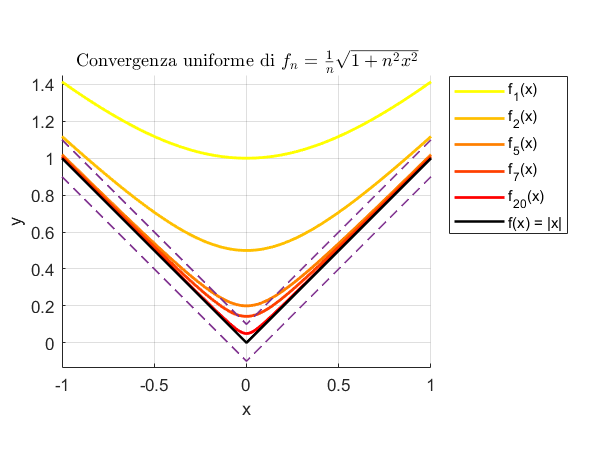
\includegraphics[width=0.39\textwidth]{Capitoli/Capitolo7/Convergenza uniforme.png}
\end{figure}
\begin{oss}
   Si può notare che la convergenza uniforme implica la convergenza puntuale, ma non è necessariamente vero il contrario.
    \end{oss}
\begin{oss}
 Per stabilire l'uniforme convergenza di una successione di funzioni, si può agire in due modi:
    \begin{itemize}
       \item Calcolare $\sup\limits_{x \in I} |\fn(x)-f(x)|$ ricercando massimi e minimi con gli strumenti del calcolo in una variabile.
       \item Maggiorare opportunamente $\sup\limits_{x \in I} |\fn(x)-f(x)|$.
\end{itemize}
\end{oss}
\begin{example}
Si studi ora la convergenza della seguente successione di funzioni, il cui grafico è riportato in figura
\begin{equation*}
    \fn= x^n, \qquad x \in [0,1]
\end{equation*}
Per quanto riguarda la convergenza puntuale si osserva che, fissato $x \in [0,1]$,
\begin{equation*}
    \lim_{n \to +\infty}{\fn(x)}= \lim_{n \to + \infty}= f(x) = \begin{cases}
        0 &\quad x \in [0,1]\\
        1 &\quad x=1
    \end{cases}
\end{equation*}
Volendo poi studiare la convergenza uniforme, si ha che
\begin{equation*}
    \sup_{x \in [0,1]}{\left|\fn(x)-f(x)\right|} = \sup_{x \in [0,1]} \left\{ \sup_{x \in [0,1)} \left|\fn(x)-f(x)\right|, \left|\fn(x)-f(x)\right|\right\} = \sup_{x \in [0,1)}{\left|x^n-0\right|} = 1 \neq 0
\end{equation*}
Dunque in $[0,1]$ $\fn$ non converge in modo uniforme. D'altra parte è anche vero che la "patologia" si verifica in $x=1$, perciò valutando la convergenza uniforme in $[0,a],\ a < 1$, si ha che
\begin{equation*}
    \sup_{x \in [0,a]}{|\fn(x)-f(x)|}= x^n \big|_{[0,a]} = a^n \overset{n \to +\infty}{\to} 0
\end{equation*}
cioè $\fn$ uniformemente convergente a $0$ su ogni compatto $[0,a],\ a<1$.\\
È possibile avere un riscontro grafico di tali affermazioni dalla figura di seguito.
\begin{figure}[H]
    \centering
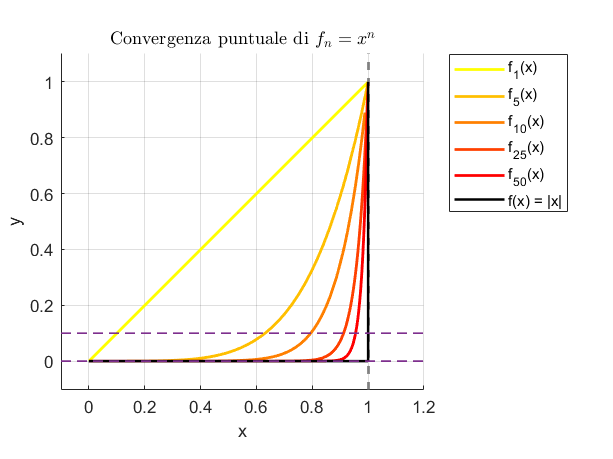
\includegraphics[width=0.55\textwidth]{Capitoli/Capitolo7/Convergenza puntuale.png}
    \end{figure}
\end{example}
\begin{theorem}[Scambio di limiti] \label{Teo: Scambio di limiti}
Sia $\fn: I \to \R$ tale che $\{\fn\}_n$ converge uniformemente in $I$ a $f: I \to \R$. Sia $x_0$ un punto di accumulazione per $I$ e si supponga che per ogni $n \in \N$ esista
\begin{equation}
    \ell_n:= \lim_{x \to x_0}{\fn(x)} \in \R
\end{equation}
Allora esistono i seguenti limiti e si ha
\begin{equation}
    \lim_{n \to +\infty}{\left(\lim_{x \to x_0} {\fn(x)}\right)}= \lim_{n \to +\infty}{\ell_n} = \lim_{x \to x_0} {f(x)} = \lim_{x \to x_0}{ \left( \lim_{n \to +\infty} {\fn(x)}\right)}
\end{equation}
\end{theorem}
\begin{proof}
    Si mostri che $\ell_n$ è una successione di Cauchy.\\
    Dalla convergenza uniforme delle $f_n$ si ha che
    \begin{equation}
        \forall\ \varepsilon>0\ \exists\ N_\varepsilon \in \N\ \text{tale che}\ \left| \fn(x)-f(x)\right|< \varepsilon,\ \forall\ x \in I
    \end{equation}
    Perciò, passando al limite per $x \to x_0$, si ha che
    \begin{equation}
        \left| \lim_{x \to x_0}{\fn(x)}-\lim_{x \to x_0}{f(x)}\right| = \left| \ell_n - \ell_m \right| \leq \varepsilon
    \end{equation}
    cioè $\ell_n$ è di Cauchy. Inoltre, $\{\ell_n\}_n$ è una successione di numeri reali, dunque essa deve convergere ad un qualche $\ell \in \R$. Ciò dimostra la prima metà della tesi.\\
    Rimane da provare che $f(x) \overset{x \to x_0}{\to} \ell$, cioè che $|f(x)-\ell| \to 0$. Dunque,
    \begin{equation}
    \begin{aligned}
        \left|f(x)-\ell\right| &= \left| f(x) - f_\nu(x)+ f_\nu(x)- \ell_\nu+ \ell_\nu- \ell\right| \leq\\
        &\overset{\text{Triang.}}{\leq} \left| f(x) - f_\nu(x) \right| +\left| f_\nu(x)- \ell_\nu(x)\right|+\left|\ell_\nu-\ell\right|
    \end{aligned}
    \end{equation}
    Si può notare che il primo termine è minore di $\varepsilon$ per ogni $\nu > N_\varepsilon$ per convergenza uniforme e che il terzo, essendo una successione numerica, è minore di $\varepsilon$ per un $\nu$ sufficientemente grande, poiché $\ell_n \to \ell$. Il secondo, fissato $\nu$ come sopra, soddisfa per ipotesi
    \begin{equation}
        \lim_{x \to x_0}{f_\nu(x)} = \ell_\nu
    \end{equation}
    Dunque, esiste un intorno $\U(x_0)$ tale che per ogni $x \in \U(x_0)$, $\left| f_\nu(x)- \ell_\nu \right| < \varepsilon$.\\
    In conclusione, per $\nu$ fissato come sopra e $x \in \U(x_0)$ si ha che
    \begin{equation}
        \left|f(x)-\ell\right| < 3 \varepsilon
    \end{equation}
\end{proof}
\begin{oss}
    Il passaggio al limite nella prima parte della dimostrazione è consentito dal fatto che per ipotesi siano definite $\ell_n$ e $\ell_m$ reali.
\end{oss}
Da tale teorema discende come conseguenza immediata il seguente corollario
\begin{corollary} \label{Cor: Corollario a scambio limiti}
    Sia $\fn$ una successione di funzioni continue uniformemente convergente in $I$ a $f:I \to \R$. Allora $f$ è continua. 
\end{corollary}
\begin{proof}
    Si mostri che preso $x_0$ punto di accumulazione per $I$, si ha
    \begin{equation}
        \lim_{x \to x_0}{f(x)}= f(x_0)
    \end{equation}
    Dunque sfruttando l'ipotesi di convergenza, si ha che
    \begin{equation}
        \lim_{x \to x_0}{\fn(x)}= \fn(x_0) \in \R
    \end{equation}
    D'altra parte vale lo scambio di limiti, quindi
    \begin{equation}
    \begin{aligned}
          f(x_0) &=  \lim_{n \to +\infty}{\fn(x_0)}= \lim_{n \to +\infty}{\left(\lim_{x \to x_0}{\fn(x)}\right)}=\\
          &= \lim_{x \to x_0}{ \left( \lim_{n \to +\infty}{\fn(x)}\right)}=\lim_{x \to x_0}{f(x)} 
    \end{aligned}
    \end{equation}
\end{proof}
Vista tale proprietà dei limiti, può essere ragionevole porsi lo stesso dubbio per le derivate e gli integrali. A tal proposito, si mostrino ora due importanti risultati rispetto alla derivazione e all'integrazione di successioni di funzioni.
\begin{theorem}[Teorema di passaggio al limite sotto al segno di derivata] \label{Teo: Passaggio al limite sotto al segno di derivata}
    Sia $\{\fn\}_{n\in\N}$ una successione di funzioni $C^1[a,b]$. Sia la successione di numeri reali $\{\fn(x_0)\}_n$ convergente e sia $\{\fn'\}_n$ uniformemente convergente. Allora $\{\fn\}_n$ converge uniformemente in $[a,b]$ ad una funzione $f \in C^1([a,b])$ e 
    \begin{equation}
        \lim_{n \to +\infty}{\fn'(x)}= \left(\lim_{n \to +\infty}{\fn(x)}\right)'=f'(x)
    \end{equation}
\end{theorem}
\begin{theorem}[Teorema di passaggio al limite sotto al segno di integrale] \label{Teo: Passaggio al limite sotto al segno di integrale}
Sia $\{\fn\}_{n_\in \N}$ una successione di funzioni continue in $[a,b]$ uniformemente convergente in $[a,b]$ a $f$. Allora
\begin{equation}
    \lim_{n \to +\infty}{\int\limits_{a}^{b}{\fn(x)}\,dx}=\int\limits_{a}^{b}{\lim_{n \to +\infty}{\fn(x)}\,dx}= \int\limits_{a}^{b}{f(x)}\,dx
\end{equation}
\end{theorem}
\begin{example}
    In questo esempio si può osservare quanto sia rilevante l'ipotesi di uniforme convergenza della successione.
    \begin{figure}[H]
        \centering
        \begin{minipage}{0.5\textwidth}
            Si consideri la successione di funzioni data da 
            \begin{equation*}
            f_n(x)=\begin{cases}
            0 &\qquad x=0\\
            n & \qquad x \in (0, \frac{1}{n})\\
            0 &\qquad x \in (\frac{1}{n}, 1)\\
            \end{cases}
            \end{equation*}
            e si osservi che
            \begin{equation*}
                \int\limits_{0}^{1}{\fn(x)}\,dx=1 \neq \int\limits_{0}^{1}{f(x)}\,dx = 0
            \end{equation*}
        \end{minipage}
        \begin{minipage}{0.4\textwidth}
        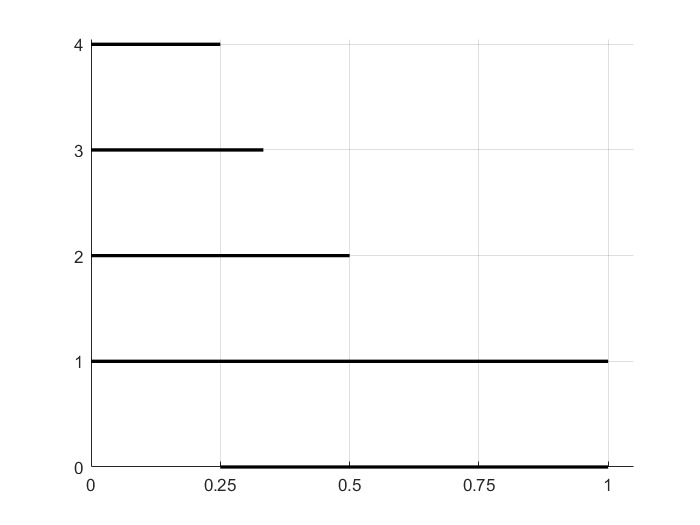
\includegraphics[width=\textwidth]{Capitoli/Capitolo7/Esempio integrale succ. funz..png}
        \end{minipage}
    \end{figure}
    poiché non uniformemente convergente.
\end{example}
\section{Serie di funzioni}
Quando si parla di serie, ci si può rifare alle successioni. Perciò in questa sezione verranno rielaborate le informazioni del capitolo precedente adattandole alle serie di funzioni.
\begin{definition}
    Sia $\{\fn\}_{n \in \N}$ una successione di funzioni, $\fn: I \subseteq \R \to \R$. Si dice \textbf{serie di funzioni} di termine generale $\fn$ la successione di funzioni delle somme parziali di $\{\fn\}_{n \in \N}$ data da
    \begin{equation}
        \sn(x)=\sum\limits_{n=1}^{N}{\fn(x)}
    \end{equation}
\end{definition}
\begin{definition}
    Sia $\sum\limits_{n=1}^{\infty}{\fn(x)}$ una serie di funzioni. Allora si dice che la serie \textbf{converge puntualmente} in I se la successione $\{\sn\}_{n \in \N}$ converge puntualmente in I. In maniera equivalente, la serie converge se, detta
    \begin{equation}
        s(x)=\lim_{n \to +\infty}{\sn(x)}
    \end{equation}
    si ha che
    \begin{equation}
        \forall\ x \in I,\ \forall\ \varepsilon>0,\ \exists\ N_{\varepsilon, x}\ \text{tale che}\ \forall N>N_{\varepsilon, x}\ \text{si ha che}\ |\sn(x)-s(x)|< \varepsilon
    \end{equation}
    o, ancora, sfruttando il criterio di Cauchy, se
    \begin{equation}
        \forall\ x \in I,\ \forall\ \varepsilon>0,\ \exists\ N_{\varepsilon, x}\ \text{tale che}\ \forall\ n>N_{\varepsilon, x},\ \forall p \in \N\ \text{si ha}\ |f_{n+1}(x)+ \dots+ f_{n+p}(x)|<\varepsilon
    \end{equation}
\end{definition}
\begin{definition}
    Se la serie converge puntualmente è ben definita la funzione \textbf{somma}
    \begin{equation}
        s(x)=\lim_{n \to +\infty}{\sn(x)}= \sum_{n=0}^{\infty}{\fn(x)}
    \end{equation}
\end{definition}
\begin{definition}
Sia $\sum\limits_{n=1}^{\infty}{\fn(x)}$ una serie di funzioni. Allora si dice che la serie \textbf{converge uniformemente} in I se la successione $\{\sn\}_{n \in \N}$ converge uniformemente in I. In maniera equivalente, sfruttando il criterio di Cauchy uniforme, se
\begin{equation}
\forall\ \varepsilon>0\ \exists\ N_\varepsilon \in \N\ \text{tale che}\ \forall\ n > N_\varepsilon\ \forall\ p \in \N\ \text{si ha}\ \sup_{x \in I}{|f_{n+1}(x)+\dots+f_{n+p}(x)|}<\varepsilon 
\end{equation}
\end{definition}
\begin{definition}
    Sia $\{\sn\}_{n \in \N}$ una serie di funzioni. Si dice che la serie \textbf{converge assolutamente}  se
    \begin{equation}
        \sum_{n}{|\fn(x)|}
    \end{equation}
    converge per ogni $x \in I$
\end{definition} 
\begin{oss}
Valgono le seguenti relazioni tra le varie nozioni di convergenza per le serie:
\begin{itemize}
    \item Convergenza assoluta $\Rightarrow$ Convergenza puntuale.
    \item  Nessuna correlazione tra convergenza assoluta e convergenza uniforme.
\end{itemize}
\end{oss}
\begin{example}
    La convergenza puntuale non implica la convergenza assoluta. Infatti, sia
    \begin{equation*}
        \fn(x)=\frac{(-1)^n}{n}
    \end{equation*}
    Allora $\sum\limits_{n}{\fn}$ converge ma $\sum\limits_{n}{|\fn|}$ diverge.
\end{example}
\begin{definition}
    Sia $\sum\limits_{n=1}^{\infty}{\fn(x)}$ una serie di funzioni. Si dice che essa converge totalmente in $I$ se esiste una successione numerica $\{k_n\}_n$ con $k_n>0$ per ogni $n$ tale che
    \begin{enumerate}
        \item $|\fn|<k_n$
        \item $\sum\limits_{n}{k_n}$ converge
    \end{enumerate}
\end{definition}
\begin{proposition}
    Una serie totalmente convergente è assolutamente convergente.
\end{proposition}
\begin{proof}
    Se $\sum\limits_{n}\fn$ converge totalmente, allora per definizione esiste una successione $k_n$ tale che $|\fn|<k_n$ e tale che la propria serie converga. Ma allora si ha che
    \begin{equation}
        \sum_{n}{|\fn|} < \sum_{n}{k_n}= \ell \in \R
    \end{equation}
    Perciò, per il teorema del confronto per le serie, $\sum\limits{|\fn|}$ converge e, quindi, $\sum\limits{\fn}$ converge assolutamente.
\end{proof}
\begin{theorem}[Criterio di Weierstrass] \label{Teo: Criterio di Weierstrass (convergenza totale)}
Una serie di funzioni $\sum\limits_{n=1}^{\infty}{\fn(x)}$ totalmente convergente in $I$ è ivi uniformemente convergente.
\end{theorem}
\begin{proof}
    Si sfrutti il criterio di Cauchy uniforme per le serie. L'obiettivo quindi è mostrare che esista un $N_\varepsilon$ tale che $|f_{n+1}+ \dots+ f_{n+p}|< \varepsilon,\ \forall\ n > N_\varepsilon,\ \forall\ p\in \N$.\\
    Dunque, si fissi $\varepsilon>0$. Per ipotesi di convergenza totale si ha che $\sum\limits_{n=1}^{\infty}{k_n}$ converge. Allora, esiste un $N_\varepsilon>0$ tale che per ogni $n>N_\varepsilon$ si ha che 
    \begin{equation}
        |k_{n+1}+\dots+k_{n+p}|< \varepsilon \qquad \forall\ p \in \N
    \end{equation}
   con $k_n>0\ \forall\ n$.\\
   D'altra parte, $|\fn|<k_n$ e, di conseguenza, a patto di prendere $n> N_\varepsilon$ si ha che, $\forall\ p \in \N,\ \forall x \in I$, vale
    \begin{equation}
    \begin{aligned}
        |f_{n+1}(x)+ \dots + f_{n+p}(x)| &\leq |f_{n+1}(x)|+ \dots + |f_{n+p}(x)|<\\ 
        &< k_{n+1}+ \dots + k_{n+p} < \varepsilon
    \end{aligned}
    \end{equation}
    Dunque è verificato il criterio di Cauchy uniforme e la serie converge uniformemente in I.
\end{proof}
\begin{oss}
    Il teorema offre una condizione sufficiente per la convergenza uniforme.
\end{oss}
\begin{oss}
Per quanto visto, una serie $\sum\limits_{n}{\fn(x)}$ converge totalmente se e solo se $\sum\limits_{n}{\sup\limits_{x \in I}{|\fn(x)|}} < +\infty$. Infatti, se in tale contesto esiste una $k_n \geq |\fn(x)|$ per ogni $n$ la cui serie converge, allora è soddisfatta la definizione di convergenza totale.\\
Anche qui si può operare in due modi:
\begin{itemize}
    \item Calcolare $\sup\limits_{x \in I}{|\fn(x)|}$.
    \item Maggiorare opportunamente $\sup\limits_{x \in I}{|\fn|}$.
\end{itemize}
\end{oss}
Con le dovute modifiche all'enunciato, valgono per le serie i teoremi \ref{Teo: Scambio di limiti}, \ref{Cor: Corollario a scambio limiti}, \ref{Teo: Passaggio al limite sotto al segno di derivata} e \ref{Teo: Passaggio al limite sotto al segno di integrale} mostrati nella sezione precedente.
\begin{theorem}[Teorema di scambio dei limiti per le serie di funzioni]
    Sia $\fn: E \subseteq \R \to \R$ e sia $x_0$ di accumulazione per $E$. Se esiste finito
    \begin{equation}
        \lim_{x \to x_0}{\fn(x)} \qquad \forall\ n\geq0
    \end{equation}
    e se $\sum\limits_{n=0}^{\infty}{\fn(x)}$ converge uniformemente su E alla somma $S(x)$, allora $S(x)$ converge per $x \to x_0$ e 
    \begin{equation}
        \lim_{x \to x_0}{S(x)= \sum\limits_{n=0}^{\infty}{\lim_{x \to x_0}{\fn(x)}}}
    \end{equation}
\end{theorem}
\begin{theorem}
    Siano $I \subseteq \R,\ \fn \in C^0(I)$ e sia $\sum\limits_{n=0}^{\infty}{\fn(x)}$ uniformemente convergente in $I$ a $s$. Allora la funzione somma $s(x)$ è continua in $I$.
\end{theorem}
\begin{theorem}
    Sia $\fn \in C^1([a,b])$ e si supponga $\sum\limits_{n=0}^{\infty}{\fn(x)}$ puntualmente convergente in $[a,b]$ a $s(x)$ e $\sum\limits_{n=0}^{\infty}{\fn'(x)}$ uniformemente convergente in $[a,b]$. Allora
    \begin{equation}
        \sum\limits_{n=0}^{\infty}{\fn'(x)}= 
        \left(\sum\limits_{n=0}^{\infty}{\fn(x)}\right)'= s'(x) \qquad \forall\ x \in [a,b]
    \end{equation}
\end{theorem}
\begin{theorem}
    Sia $\fn \in C^0([a,b])$ e sia $\sum\limits_{n=0}^{\infty}{\fn(x)}$ uniformemente convergente in $[a,b]$ a $s$. Allora
    \begin{equation}
        \sum\limits_{n=0}^{\infty}{\int\limits_{a}^{b}{\fn(x)}\, dx}= \int\limits_{a}^{b}{\sum\limits_{n=0}^{\infty}{\fn(x)}\, dx}= \int\limits_{a}^{b}{s(x)}\, dx
    \end{equation}
\end{theorem}
\section{Serie di potenze}
\begin{definition}
Si dice \textbf{serie di potenze} reale di centro $x_0 \in \R$ una serie di funzioni della forma
\begin{equation}
    a_0+ \sum_{n=1}^{\infty}{a_n(x-x_0)^n} \qquad a_n \in \R\ \forall\ n=0,1,\dots
\end{equation}
\end{definition}
\begin{oss}
    Mediante opportune traslazioni è possibile passare da una serie di potenze centrata in $x_0$ a una centrata in $0$ della forma
    \begin{equation}
        \sum_{n=0}^{\infty}{a_n x^n}
    \end{equation}
\end{oss}
\begin{definition}
    Si dice \textbf{raggio di convergenza} della serie $\sum\limits_{n=0}^{\infty}{a_n x^n}$ l'estremo superiore $R$ dell'insieme $E$ dei numeri reali $\xi$ nei quali la serie converge, ossia
    \begin{equation}
        R= \sup E \qquad E=\left\{ \xi \in \R \mid \sum_{n=0}^{\infty}{a_n x^n}\ \text{converge}\right\}
    \end{equation}
\end{definition}
La caratterizzazione di $R$ si ha a partire dal seguente teorema.
\begin{theorem} \label{Teo: Caratterizzazione del raggio di convergenza}
    Sia $R$ raggio di convergenza della serie di potenze. Se $R=0$, allora la serie converge solo in $0$. Se $R>0$, la serie converge totalmente in ogni $[a,b] \subset (-R, R)$ e non converge per $|x|>R$.
\end{theorem}
\begin{proof}
 Si mostri che se $\sum\limits_{n=0}^{\infty}{a_n \xi^n}$ converge per un qualche $\xi \neq 0$ allora converge totalmente in ogni intervallo $[-\eta, \eta] \subset (-|\xi|, |\xi|)$.\\
 Per ipotesi di convergenza della serie, $|a_n \xi^n|$ deve essere una successione infinitesima (e perciò limitata) per $n\to +\infty$, ovvero
 \begin{equation}
     \exists\ M>0\ \text{tale che}\ |a_n\xi^n|\leq M
 \end{equation}
 A questo punto, fissato $\eta>0$ tale che $\eta<|\xi|$, si calcoli il termine generale della serie per un qualche $x \in [-\eta, \eta]$.
 \begin{equation}
     |a_n x^n| = \left|a_n x^n \frac{\xi^n}{\xi^n}\right|=\left|a_n \xi^n\right| \left|\frac{x}{\xi}\right|^n \leq M \left(\frac{|x|^n}{\left|\xi\right|^n} \right)\leq M \left(\frac{\eta}{\left| \xi \right|} \right)^n =k_n
 \end{equation}
 Poiché $k_n$ è il termine generale di una serie geometrica di ragione $\left(\tfrac{\eta}{\left| \xi \right|} \right)^n < 1$, essa è convergente. Quindi
 \begin{equation}
 \forall\ x \in [-\eta, \eta],\ \sum\limits_{n=0}^{\infty}{|a_n \xi^n|} \leq M \sum_{n=0}^{\infty}{\left(\frac{\eta}{\left| \xi \right|} \right)^n}
 \end{equation}
 che soddisfa le condizioni di convergenza totale con $k_n=\left(\tfrac{\eta}{\left| \xi \right|} \right)^n$.\\
 Nel caso in cui $R=0$, per quanto detto, la serie non può convergere in punti $\xi$ tali che $\xi \neq 0$.\\
 Nel caso in cui $|x|>R$, si ha che, per $x>R$ la serie non converge perché andrebbe in contraddizione con la definizione di $\sup$ propria di $R$; discorso analogo vale per $x<-R$, siccome la convergenza in tale punto implicherebbe la convergenza in ogni $[-\eta, \eta] \subset (-|x|, |x|)$ e, se così fosse, si contraddirebbe nuovamente la definizione di $\sup$.
\end{proof}
\begin{oss}
Il teorema dà un'ulteriore informazione: se $R= +\infty$, allora la serie di potenze converge totalmente in ogni compatto di $\R$.
\end{oss}
\begin{theorem}[Criterio di Cauchy-Hadamard] \label{Teo: Criterio di Cauchy-Hadamard}
Sia $\sum\limits_{n=0}^{\infty}{a_n x^n}$ una serie di potenze. Se esiste il limite
\begin{equation}
    \ell=\lim_{n \to +\infty}{\sqrt[n]{|a_n|}}
\end{equation}
    allora il raggio di convergenza vale
    \begin{equation}
        R = \begin{cases}
            +\infty &\qquad \ell=0\\
            \frac{1}{\ell} &\qquad \ell \neq 0\\
            0 &\qquad \ell = +\infty
        \end{cases}
    \end{equation}
\end{theorem}
\begin{proof}
    Per ogni $x \neq 0$ risulta
    \begin{equation}
        \lim_{n \to +\infty}{\sqrt[n]{|a_n x^n|}} = \ell|x| := L
    \end{equation}
    Allora, dallo studio di $\ell$ si ha che
    \begin{enumerate}
        \item $\ell=0 \Rightarrow L=0$, perciò, per criterio della radice delle serie numeriche, la serie converge assolutamente per ogni $x \neq 0$. Inoltre, poiché la serie converge anche con $x=0$, $R=+\infty$.
        \item $\ell= +\infty \Rightarrow L =+ \infty$, quindi, per ogni $x \neq 0$ la serie non converge assolutamente, cioè $R=0$.
        \item $0< \ell<+\infty$, per il criterio della radice delle serie numeriche, quando $L<1 \iff |x|< \tfrac{1}{\ell}$ la serie converge assolutamente. Invece, quando $L>1 \iff |x|>\tfrac{1}{\ell}$ la serie non converge assolutamente, quindi, $R= \tfrac{1}{\ell}$.
    \end{enumerate}
\end{proof}
Oltre al criterio della radice, vale anche il criterio del rapporto, di cui viene dato solo l'enunciato, dal momento che la sua dimostrazione è analoga a quella precedente con l'eccezione di applicare il criterio del rapporto per le serie numeriche anziché quello della radice.
\begin{theorem}[Criterio di d'Alembert]
    Sia $\sum\limits_{n=0}^{\infty}{a_n x^n}$ una serie di potenze. Se esiste il limite
    \begin{equation}
        \ell= \lim_{n \to \infty}{\frac{a_{n+1}}{a_n}}
    \end{equation}
    allora il raggio di convergenza della serie vale
    \begin{equation}
        R= \begin{cases}
        +\infty &\qquad \ell=0\\
        \frac{1}{\ell} &\qquad \ell \neq 0\\
        0 &\qquad \ell = \infty
        \end{cases}
    \end{equation}
\end{theorem}
Il teorema di Abel, che segue, offre una condizione sufficiente per la convergenza uniforme di serie di potenze.
\begin{theorem}[Teorema di Abel] \label{Teo: Teorema di Abel}
    Sia $\sum\limits_{n=0}^{\infty}{a_n x^n}$ una serie di potenze con raggio di convergenza $R$, con $0<R<+\infty$. Sia poi $M$ tale che $0<M<R$. Se la serie converge anche in $x=R$ (o $x=-R$) allora la serie converge uniformemente su $[-M, R]$ (o $[-R, M]$). \\
    In particolare, se la serie converge in $x= \pm R$, allora essa converge uniformemente in $[-R, R]$.
\end{theorem}
\subsection{Sviluppabilità di una funzione in serie di potenze}
\begin{theorem}[Derivazione di serie di potenze] \label{Teo: Derivazione di serie di potenze}
Sia $\sum\limits_{n=0}^{\infty}{a_n x^n}$ una serie di potenze con raggio di convergenza $R>0$. Sia poi $f$ la sua funzione somma. Allora la serie
\begin{equation}
    \sum\limits_{n=1}^{\infty}{\left(a_n x^n\right)'}= \sum\limits_{n=1}^{\infty}{n a_n x^{n-1}}= \sum\limits_{j=0}^{\infty}{\left(j+1\right)a_{j+1} x^j}
\end{equation}
ha lo stesso raggio di convergenza $R$. Inoltre, esiste $f'(x)\ \forall\ x \in (-R, R)$ e
\begin{equation}
    f'(x)=\sum\limits_{n=0}^{\infty}{\left(n+1\right)a_{n+1} x^n}
\end{equation}
\end{theorem}
\begin{proof}
    Per semplicità si supponga che esista e valga 
    \begin{equation}
        \lim_{n \to \infty}{\sqrt[n]{|a_n|}}=\frac{1}{R}
    \end{equation}
    e si calcoli il raggio di convergenza della serie derivata. Allora
    \begin{equation}
        \lim_{j \to + \infty}{\sqrt[j]{(j+1)|a_{j+1}|}} = \lim_{j \to + \infty}{\sqrt[j]{(j+1)}} \lim_{j \to + \infty}{\sqrt[j]{|a_{j+1}|}}= \lim_{j \to + \infty}{{\left(|a_{j+1}|^{\frac{1}{j+1}}\right)^{\frac{j+1}{j}}}}  \overset{\ref{Teo: Criterio di Cauchy-Hadamard}}{=} \frac{1}{R}
    \end{equation}
    E quindi, ponendosi in un compatto $[a,b] \subset (-R, R)$ in cui la serie derivata e la serie di potenze convergono totalmente e applicando il teorema, si ha la tesi.
\end{proof}
Reiterando tale procedimento, si può osservare che la somma della serie di potenze deve essere di classe $C^\infty$. Dunque, si può stabilire una condizione necessaria di buona approssimazione di una funzione $f$ tramite una serie di potenze, cioè il fatto che $f \in C^{\infty}$. Tale questione non si pone invece parlando di serie di Fourier.\\
D'altro canto, si possono introdurre ora le serie di Taylor. 
\begin{proposition}
Sia $x_0=0$ e sia $f \in C^\infty$ tale che in $(-R, R)$ si abbia
\begin{equation}
    f(x)= \sum\limits_{n=0}^{\infty}{a_n x^n}
\end{equation}
Allora tale serie è la serie di Taylor di $f$.
\end{proposition}
\begin{proof}
Per quanto detto nel teorema precedente, deve valere
\begin{equation}
    f^{(m)}(x)= \sum\limits_{n=m}^{\infty}{\frac{n!}{(n-m)!} a_n x^{n-m}}
\end{equation}
e quindi, ponendo $x=0$, tutti gli addendi dopo il primo si azzerano, lasciando così
\begin{equation}
    f^{(m)}(0)=a_n m! \Rightarrow a_n=\frac{f^{(m)}}{m!} \qquad \forall\ n
\end{equation}
cioè $a_n$ è il coefficiente di Taylor.
\end{proof}
\begin{definition} \label{Def: Funzione analitica}
    Si dice che una funzione $f$ è una funzione \textbf{analitica} in $\U(0)$ se sull'intervallo $(-\varrho, \varrho)$ si ha che
    \begin{equation}
        f(x)= \sum\limits_{n=0}^{\infty}{a_n x^n}
    \end{equation}
\end{definition}
\begin{oss}
    Esistono funzioni di classe $C^\infty$ la cui serie di Taylor abbia raggio di convergenza $R=0$.
\end{oss}
\begin{oss}
    La definizione di funzione analitica può essere formulata in un generico $\U(x_0)$ e si può dimostrare che se $f$ è analitica in $(x_0-\varrho, x_0+\varrho)$, allora lo è anche in un intorno di ogni $x_1 \in (x_0-\varrho, x_0+\varrho)$.
\end{oss}
\begin{theorem}
    Le funzioni analitiche sono un sottoinsieme proprio di $C^\infty$
\end{theorem}
\begin{proof}
 Si dimostri il teorema con un controesempio. Sia 
 \begin{equation}
     f(x)= \begin{cases}
         e^{-\frac{1}{x^2}} &\qquad x \neq 0\\
         0 &\qquad x=0
     \end{cases}
 \end{equation}
 Tale funzione è continua in $\R$ e verifica 
 \begin{equation}
     \lim_{x \to 0}{f(x)}=0= \lim_{x \to 0}{ e ^{-\frac{1}{x^2}}}
 \end{equation}
 Allora, calcolandone la derivata prima si ha 
 \begin{equation}
     f'(x)= \begin{cases}
         \frac{2}{x^3} e^{-\tfrac{1}{x^2}} & \qquad x \neq 0\\
         \lim\limits_{x \to 0}{\frac{f(x)-f(0)}{x}}= \lim\limits_{x \to 0}{\frac{e^{-\frac{1}{x^2}}}{x}}=0 &\qquad x=0
     \end{cases}
 \end{equation}
 Continuando a derivare, si ottiene sempre un'equazione del tipo
 \begin{equation}
     f^{(m)}(x)=\begin{cases}
         C e^{-\frac{1}{x^2}} &\qquad x\neq0\\
         0 &\qquad x=0
     \end{cases}
 \end{equation}
 cioè, $f \in C^\infty(\R)$. Tuttavia, $f^{(m)}(0)=0$. Pertanto la serie di Taylor dovrebbe essere la funzione nulla, ma $f \not\equiv 0\ \forall\ x \in \dot{\U}(0)$, quindi non è analitica.
\end{proof}
Allora, per terminare, si dia ora un criterio per stabilire se una funzione sia sviluppabile come serie di potenze.
\begin{theorem}[Criterio di sviluppabilità] \label{Teo: Criterio di sviluppabilità}
    Sia $f \in C^\infty(-\varrho, \varrho)$ per un qualche $\varrho>0$. Sia poi
    \begin{equation}
        \sup_{x \in (-\varrho, \varrho)}{|f^{n}(x)|}\leq L^{n+1}n!
    \end{equation}
    per un'opportuna costante $L>0$. Allora $f$ è analitica in un intorno $\U(0)$
\end{theorem}
\begin{oss}
    Funzioni come $e^x,\ \sin(x), \ \cos(x)$ sono analitiche.
\end{oss}
\section{Spazi metrici}
\begin{definition} \label{Def: Spazi metrici}
    Sia $X$ un insieme e sia $d$ una metrica (\ref{Def: Distanza}). Si dice \textbf{spazio metrico} la coppia $\left(X, d\right)$
\end{definition}
\begin{example}
    Esempi di spazi metrici possono essere:
    \begin{itemize}
        \item $X=\R^n$ con distanza euclidea $d(x, y):= \sqrt{ \sum\limits_{i=1}^n{(x_i-y_i)^2}}$.
        \item $X=\R^n$ con $d_\infty(x,y):= \max\limits_{i=1, \dots, n}{|x_i-y_i|}$.
        \item $X=C^0([a,b], d_\infty)$ con $d_\infty(x,y):= \sup\limits_{x \in [a,b]}{|f(x)-g(x)|}$. 
    \end{itemize}
\end{example}
\begin{definition} \label{Def: Palla di raggio r}
    Sia $(X, d)$ uno spazio metrico. Si dice \textbf{palla} di raggio $r$ centrata in $x_0$ l'insieme
    \begin{equation}
    B_r(x_0)= \left\{ x \in X \mid d(x_0, x)< r\right\}
    \end{equation}
\end{definition}
\begin{definition} \label{Def: Convergenza e convergenza di Cauchy}
Una successione $\{x_n\}_n$ con $x_n \in (X, d)$ per ogni n e con $(X, d)$ spazio metrico \textbf{converge} a $x_0 \in X$ se
\begin{equation}
    d(x_n, x_0) \overset{n \to +\infty}{\to} 0
\end{equation}
Inoltre, se 
\begin{equation}
    \forall\ \varepsilon>0\ \exists\ N_\varepsilon\ \text{tale che}\ \forall\ n,m > N_\varepsilon\ \text{si ha}\ d(x_n, x_m)< \varepsilon
\end{equation}
allora tale successione è detta \textbf{di Cauchy}.
\end{definition}
\begin{definition} \label{Def: Spazio metrico completo}
    Uno spazio metrico $(X, d)$ è detto \textbf{completo} se ogni successione di Cauchy in X converge ad un elemento di X.
\end{definition}
\begin{example}
    Esempi di spazi metrici completi possono essere
    \begin{itemize}
        \item $X=\R^n$ con distanza euclidea o con $d_\infty$.
        \item $X=\R^n$ con $d_p= \left(\sum\limits_{i=1}^{n}{|x_i - y_i|^p}\right)^{\frac{1}{p}}$ e $p\geq 1$. (Nota: per $p=2$, la distanza $d_p$ è la distanza euclidea).
    \end{itemize}
    Uno spazio metrico non completo è invece $\mathbb{Q}^n$.
\end{example}
\begin{oss}
    Uno spazio vettoriale normato ($\Rightarrow$ metrico con $d(x, y)= |x-y|$) completo è detto spazio di \textbf{Banach}.\\
    Se in aggiunta la norma di tale spazio discende da un prodotto scalare, esso è detto spazio di \textbf{Hilbert}.
\end{oss}
\begin{theorem}
    $(C^0([a,b]), d_\infty)$ è uno spazio metrico completo.
\end{theorem}
\begin{proof}
    Sia $\{\fn\}_n$ di Cauchy in $(C^0([a,b]), d_\infty)$. Allora, 
    \begin{equation}
          \forall\ \varepsilon>0\ \exists\ N_\varepsilon\ \text{tale che}\ \forall\ n,m > N_\varepsilon\ \text{si ha}\ d(\fn, f_m)< \varepsilon
    \end{equation}
    cioè 
    \begin{equation}
     \sup\limits_{x \in [a,b]}{|\fn(x)-f_m(x)|}< \varepsilon
    \end{equation}
    Ma allora $\fn$ soddisfa il criterio di Cauchy uniforme ed esiste una funzione limite $f$ cui $\fn$ converge uniformemente in $[a,b]$ per $n \to \infty$. Poiché poi $\fn$ sono continue per ipotesi e convergono uniformemente ad $f$, sono soddisfatte le ipotesi del corollario \ref{Cor: Corollario a scambio limiti}, quindi $f \in C^0([a,b], d_\infty)$.
\end{proof}
\begin{oss}
    Si può notare che la definizione di completezza dipende dalla distanza. A tal proposito si consideri lo spazio metrico $(C^0([-1,1], d_p)$ con 
    \begin{equation*}
        d_p=\left(\int\limits_{-1}^{1}{|f(x)-g(x)|^p\, dx}\right)^\frac{1}{p}
    \end{equation*}
    e si prenda la successione
    \begin{equation*}
        \fn(x) = \begin{cases}
            -1 &\qquad x \in [-1, -\frac{1}{n}]\\
            nx &\qquad x \in [-\frac{1}{n}, \frac{1}{n}]\\
            1 &\qquad x \in [\frac{1}{n}, 1]
        \end{cases}
    \end{equation*}
    Il suo limite è
    \begin{equation*}
        f(x)= \sgn(x)=\begin{cases}
            -1 &\qquad x \in [-1,0)\\
            0 &\qquad x =0\\
            1 &\qquad x \in (0, 1]
        \end{cases}
    \end{equation*}
    e $f\notin C^0([-1, 1])\ \forall\ x$
    benché $\fn$ sia di Cauchy. Infatti, 
    \begin{equation*}
        d_p(\fn, f)=  d_p=\left(\int\limits_{-1}^{1}{|\fn-f|^p\, dx}\right)^\frac{1}{p} \leq \left(\int\limits_{-\tfrac{1}{n}}^{\tfrac{1}{n}}{2^p\, dx}\right)^\frac{1}{p} \overset{n \to \infty}{\to }0
    \end{equation*}
\end{oss}
\begin{definition} \label{Def: Spazio chiuso}
    Sia $(X, d)$ metrico. Un sottoinsieme $C \subset X$ è detto \textbf{chiuso} se ogni successione $\{x_n\}_n$ di elementi di $C$ che converge rispetto a $d$, converge ad un elemento di $C$.
\end{definition}
\begin{theorem} \label{Teo: Sottospazio chiuso di un completo è completo}
    Sia $(X,d)$ uno spazio metrico completo e $C \subset X$ chiuso. Allora $(C, d)$ è un sottospazio metrico completo.
\end{theorem}
\begin{proof}
    Sia $\{x_n\}_n$ una successione di Cauchy in $C$. Poiché $x_n \in C \subset X$ e $X$ è metrico completo, 
    \begin{equation}
        \exists\ y \in X\ \text{tale che}\ d(x_n, y)\to 0
    \end{equation}
    D'altra parte $x_n$ è una successione di $C$, che è chiuso. Dunque, per definizione, $y \in C$, cioè $C$ è metrico completo.
\end{proof}
\begin{definition} \label{Def: Funzione sequenzialmente continua}
    Siano $(X, d_x),\ (Y, d_y)$ spazi metrici. Allora $f: X \to Y$ è detta \textbf{sequenzialmente continua} in $x_0 \in X$ se per ogni successione $\{x_n\}_n \subset X$ tale che $x_n \overset{n\to +\infty}{\to} x_0$ rispetto a $d_x$, si ha che $f(x_n) \to f(x_0)$ rispetto a $d_y$.
\end{definition}
\begin{definition} \label{Def: Lipschitziana}
     Siano $(X, d_x),\ (Y, d_y)$ spazi metrici. Allora $f: X \to Y$ è detta \textbf{Lipschitziana} con costante di Lipschitz $L>0$ se 
     \begin{equation}
         d_y(f(x_1), f(x_2)) \leq L\,d_x(x_1, x_2) \qquad \forall\ x_1, x_2\in X
     \end{equation}
    \end{definition}
\begin{definition} \label{Def: Contrazione}
     Se $(Y, d_y)=(X, d_x)$, $0<L<1$ e $f$ come sopra, allora $f$ è detta \textbf{contrazione}.
\end{definition}
\begin{theorem}[Teorema delle contrazioni o di Banach-Caccioppoli] \label{Teo: delle contrazioni}
    Siano $(X, d_x)$ metrico completo e $f: X \to X$ contrazione. Allora 
    \begin{equation}
    \exists!\ \overline{x} \in X \text{tale che}\ f(\overline{x})=\overline{x} 
    \end{equation}
    Tale punto è detto \textbf{punto fisso}.
\end{theorem}
\begin{proof}
    Si parta dal mostrare l'esistenza di tale $\overline{x}$.\\
    Sia $x_0 \in X$ arbitrario e si costruisca una successione $\{x_n\}_n \subset X$ tale che per ogni $n$:
    \begin{equation}
            x_1=f(x_0),\ x_2=f(x_1),\ \dots\ ,\ x_{n+1}=f(x_n)
    \end{equation}
    e si mostri che essa è di Cauchy. Vale
    \begin{equation}
    \begin{aligned}
        d(x_2, x_1)=d(f(x_1), f(x_0)) &\overset{\text{Contr.}}{\leq} L\, d(x_1, x_0) = L\, d(f(x_0), x_0)\\
        d(x_3, x_2)=d(f(x_2), f(x_1)) &\overset{\text{Contr.}}{\leq} L\, d(x_2, x_1) = L^2\,d(f(x_0), x_0)\\
        &\vdots\\
        d(x_{n+1}, x_n)= d(f(x_n), f(x_{n-1}))&\overset{\text{Contr.}}{\leq} L\, d(x_n, x_{n-1}) = L^n\,d(f(x_0), x_0)
    \end{aligned}
    \end{equation}
    In generale
    \begin{equation}
    \begin{aligned}
        d(x_{n+p}, x_n) &\leq d(x_n, x_{n+1})+ d(x_{n+1}, x_{n+2})+ \dots+ d(x_{n+p-1}, x_{n+p}) \leq\\
        &\leq L^n\,d(x_0, f(x_0))+ L^{n+1}\, d(x_0, f(x_0))+ \dots+ L^{n+p-1}\, d(x_0, f(x_0))=\\
        &=L^n(1+L+\dots+L^{p-1})\,d(x_0, f(x_0)) \overset{\text{S. geom.}}{=} L^n \frac{1-L^p}{1-L}\, d(x_0, f(x_0)) \leq\\
        &\leq \frac{L^n}{1-L}\, d(x_0, f(x_0)) \to 0
    \end{aligned}
    \end{equation}
    cioè $\{x_n\}_n$ è di Cauchy. Tuttavia, essendo $(X, d)$ metrico completo per ipotesi, è verificata l'esistenza di $\overline{x} \in X$ tale che $x_n \to \overline{x}$ rispetto a $d$.\\
    Occorre ora mostrare che $\overline{x}$ è un punto fisso di $f$.\\
    Si parta dal considerare 
    \begin{equation}
        x_{n+1}=f(x_n) \qquad \forall\ n
    \end{equation}
    Passando al limite per $n \to +\infty$ ad ambo i membri si ha
    \begin{equation}
        \overline{x}= \lim_{n \to +\infty}{x_{n+1}}=\lim_{n \to +\infty}{f(x_n)} = f(\overline{x})
    \end{equation}
    poiché $f$ è una contrazione ed è perciò Lipschitziana e di conseguenza sequenzialmente continua. Perciò, $\overline{x}$ è un punto fisso.\\
    Si mostri infine l'unicità di tale punto fisso.\\
    Per assurdo si ipotizzi l'esistenza di un secondo punto fisso $y \neq \overline{x}$. Si calcoli allora la distanza tra i due
    \begin{equation}
        d(\overline{x}, y)= d(f(\overline{x}), f(y)) \leq L\, d(\overline{x}, y)
    \end{equation}
    Allora deve essere 
    \begin{equation}
        (1-L)\, d(\overline{x}, y) \leq 0
    \end{equation}
    e, poiché $(1-L)>0\ \forall\ L$ e $d(x, y) \geq 0\ \forall\ x,y$, tale relazione è soddisfatta solo se
    \begin{equation}
        d(\overline{x}, y)=0
    \end{equation}
    cioè $\overline{x}=y$.
\end{proof}